% This must be in the first 5 lines to tell arXiv to use pdfLaTeX, which is strongly recommended.
\pdfoutput=1
% In particular, the hyperref package requires pdfLaTeX in order to break URLs across lines.

\documentclass[11pt]{article}

% Remove the "review" option to generate the final version.
\usepackage[review]{ACL2023}
\usepackage{booktabs}
\usepackage[normalem]{ulem}
\useunder{\uline}{\ul}{}

% Standard package includes
\usepackage{times}
\usepackage{latexsym}

% For proper rendering and hyphenation of words containing Latin characters (including in bib files)
\usepackage[T1]{fontenc}
% For Vietnamese characters
% \usepackage[T5]{fontenc}
% See https://www.latex-project.org/help/documentation/encguide.pdf for other character sets

% This assumes your files are encoded as UTF8
\usepackage[utf8]{inputenc}

% This is not strictly necessary, and may be commented out.
% However, it will improve the layout of the manuscript,
% and will typically save some space.
\usepackage{microtype}

% This is also not strictly necessary, and may be commented out.
% However, it will improve the aesthetics of text in
% the typewriter font.
\usepackage{inconsolata}

\usepackage{graphicx}

% If the title and author information does not fit in the area allocated, uncomment the following
%
%\setlength\titlebox{<dim>}
%
% and set <dim> to something 5cm or larger.

\title{NNTI Project Report}
\author{
  Muhammad Haris Owais Ahmed, 7059141 \\
  {\bf Ahmed Tarek Ahmed Sabek, 7059155} \\
  {\bf Mohammad Ovais, 7043719} \\
}

  
% Author information can be set in various styles:
% For several authors from the same institution:
% \author{Author 1 \and ... \and Author n \\
%         Address line \\ ... \\ Address line}
% if the names do not fit well on one line use
%         Author 1 \\ {\bf Author 2} \\ ... \\ {\bf Author n} \\
% For authors from different institutions:
% \author{Author 1 \\ Address line \\  ... \\ Address line
%         \And  ... \And
%         Author n \\ Address line \\ ... \\ Address line}
% To start a seperate ``row'' of authors use \AND, as in
% \author{Author 1 \\ Address line \\  ... \\ Address line
%         \AND
%         Author 2 \\ Address line \\ ... \\ Address line \And
%         Author 3 \\ Address line \\ ... \\ Address line}



\begin{document}

{\makeatletter\acl@finalcopytrue
  \maketitle
}
\begin{abstract}
This project report outlines tasks focused on exploring language representation models using the Hugging Face Transformers library. Initially, the report covers tasks such as dataset loading, tokenization, and inference mode with pre-trained models XGLM and GPT-2, followed by a comparative analysis between the two in terms of language modeling loss. Subsequently, multi-lingual representation space exploration involves obtaining and visualizing hidden representations using PCA and tSNE. Finally, language model adaptation for Ayacucho Quechua is addressed through various adaptation approaches, including full fine-tuning and parameter-efficient methods like bitfit, LoRA, and iA3, with a focus on performance and runtime comparison, all while leveraging Weights and Biases for logging and monitoring.
\end{abstract}

\section{Introduction}

In recent years, natural language processing (NLP) research has been propelled by advancements in pre-trained language models and access to vast datasets. The utilization of large-scale pre-trained models, such as those provided by Hugging Face Transformers, has become commonplace in various NLP tasks due to their ability to capture intricate linguistic patterns. Additionally, the availability of multilingual datasets has enabled researchers to explore language models' capabilities across diverse linguistic contexts.

This project comprises three main tasks aimed at exploring and improving language model performance using state-of-the-art techniques. 

\textbf{Task 1: Hugging Face Transformers Introduction}: Use the Hugging Face Transformers library for dataset handling and pre-trained language model usage, focusing on exploring XGLM and GPT-2 models for various languages.

\textbf{Task 2: Multi-lingual Representation Exploration}: Visualizing hidden representations of language models using dimensionality reduction techniques like PCA and tSNE, providing insights into hierarchical feature representations.

\textbf{Task 3: Low-resource Language Model Adaptation}: Adapting language models for low-resource languages, excluding the flores dataset, by exploring alternative datasets and fine-tuning approaches for enhanced language modeling performance.

\section{Task 1: Familiarization with Hugging Face Transformers and Datasets}

\subsection{Methodology}

In Task 1, we familiarized ourselves with the Hugging Face Transformers library and dataset handling, focusing on the Flores dataset, which offers diverse linguistic data. Utilizing XGLM and GPT models, we compared their performance by calculating language modeling loss metrics on training and test datasets for each language in our subset. This evaluation provided insights into the models' generalization capabilities across different linguistic domains, aiding our understanding of their effectiveness for multilingual NLP tasks.

\subsection{Results}

\begin{figure}[ht]
\centering
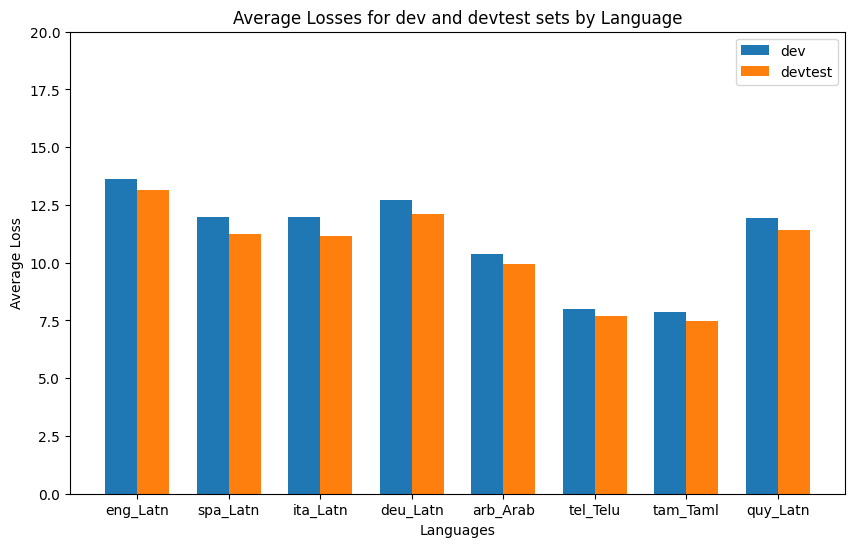
\includegraphics[width=0.9\columnwidth]{task1_xglm_results.png}
\caption{Cross-entropy loss comparison across different languages using XGLM.}
\end{figure}

\begin{figure}[ht]
\centering
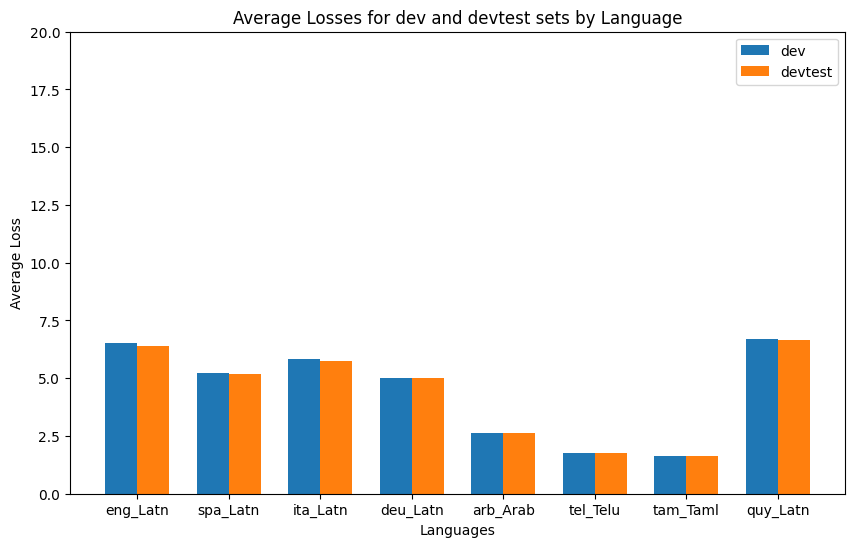
\includegraphics[width=0.9\columnwidth]{task1_gpt2_results.png}
\caption{Cross-entropy loss comparison across different languages using GPT2.}
\end{figure}

\begin{figure}[ht]
\centering
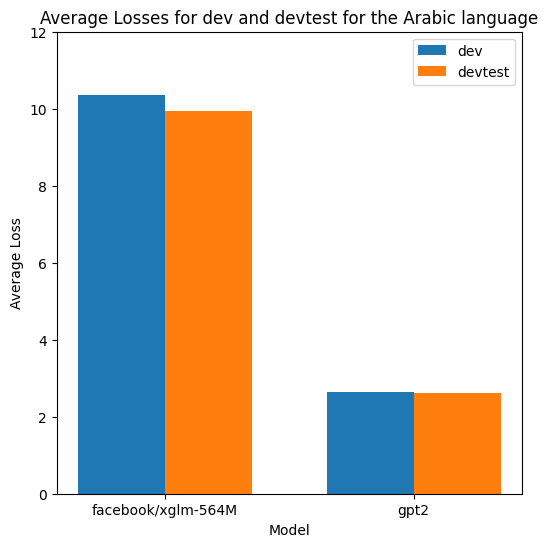
\includegraphics[width=0.9\columnwidth]{task1_modelComparison.png}
\caption{Cross-entropy loss comparison on Arabic between XGLM and GPT2.}
\end{figure}

Our analysis revealed that GPT-2 consistently exhibited smaller language modeling losses compared to XGLM across all languages in both the training and test datasets (See Figure 1 vs Figure 2, see also Figure 3).

The superior performance of GPT-2 can be attributed to several factors. Firstly, GPT-2 is a larger and more parameter-rich model compared to XGLM, allowing it to capture more complex linguistic patterns and dependencies. Additionally, GPT-2 was pre-trained on a massive corpus of text data in multiple languages, enabling it to learn robust representations across diverse linguistic domains. In contrast, XGLM may face challenges in modeling languages with limited training data or linguistic peculiarities not adequately captured during pre-training.

Furthermore, the architecture of GPT-2, specifically its transformer-based design, may offer advantages in modeling sequential data compared to XGLM. The self-attention mechanism employed in transformers allows GPT-2 to efficiently capture long-range dependencies in text sequences, contributing to its superior performance in language modeling tasks.

\section{Task 2: Exploring multi-lingual representation spaces}

\subsection{Methodology}

Principal Component Analysis (PCA) and t-Distributed Stochastic Neighbor Embedding (tSNE) are vital dimensionality reduction techniques, transforming high-dimensional feature representations into lower-dimensional spaces while preserving essential structure and relationships among data points. Leveraging PCA and tSNE provides valuable insights into multi-lingual representation spaces, enabling exploration and analysis of language models' capabilities across diverse linguistic contexts.

We performed both PCA and tSNE on two levels of visualizations:
First, visualizing token hidden representations and mean pooled token representations (mean pooled sentences) for one selected sample of sentence from the English language, and second, visualizing all mean pooled sentences from all languages together on each layer.

\subsection{Visualizations (one sentence one language)}

\begin{figure}[ht]
\centering
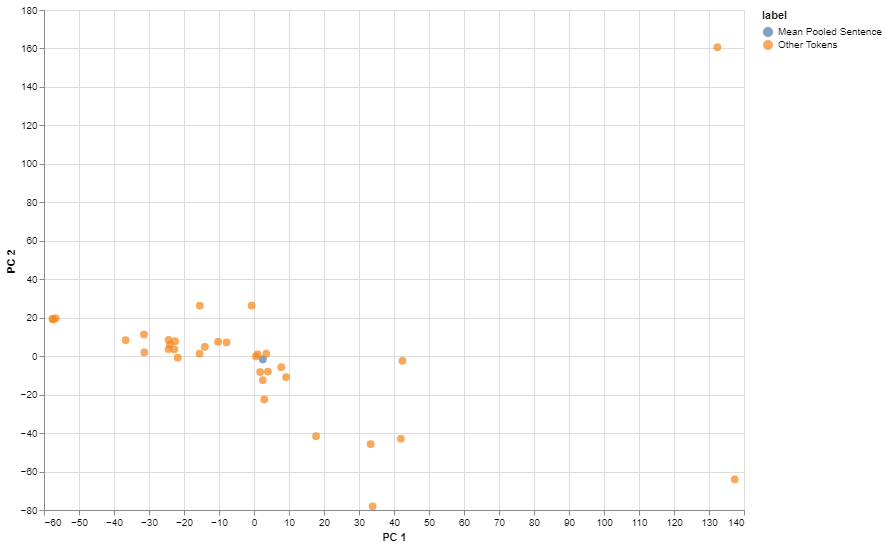
\includegraphics[width=0.9\columnwidth]{oneSentenceLang_firstLayer_pca.png}
\caption{PCA visualization of one selected sentence of one selected language on 1st layer.}
\end{figure}


\begin{figure}[ht]
\centering
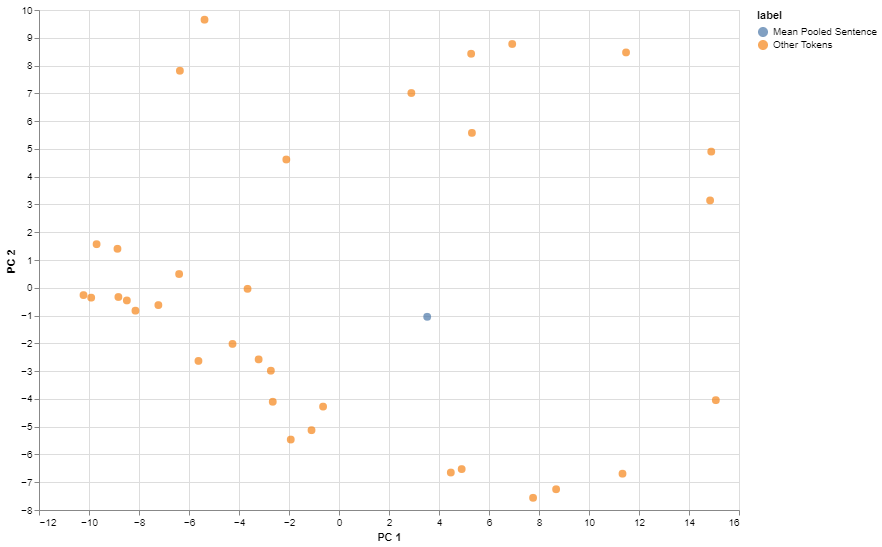
\includegraphics[width=0.9\columnwidth]{oneSentenceLang_lastLayer_pca.png}
\caption{PCA visualization of one selected sentence of one selected language on last layer.}
\end{figure}


\begin{figure}[ht]
\centering
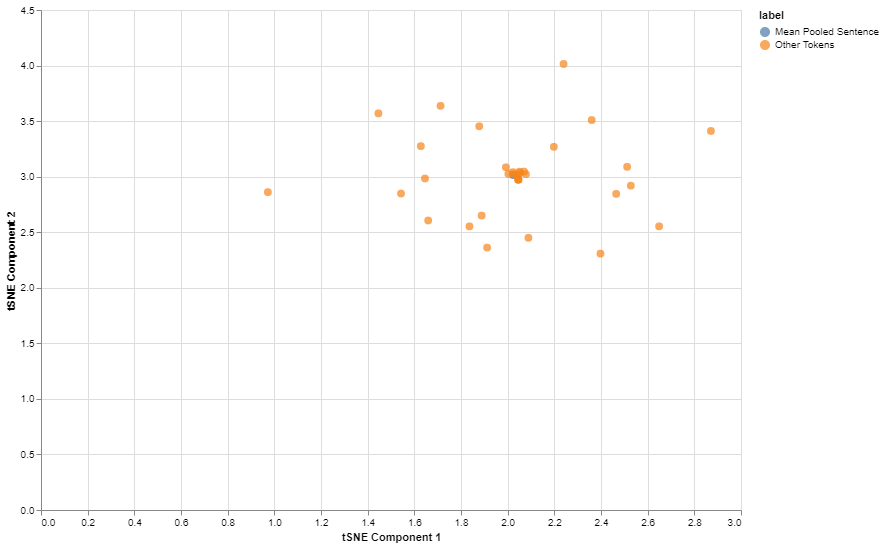
\includegraphics[width=0.9\columnwidth]{oneSentenceLang_firstLayer_tsne.png}
\caption{tSNE visualization of one selected sentence of one selected language on 1st layer.}
\end{figure}


\begin{figure}[ht]
\centering
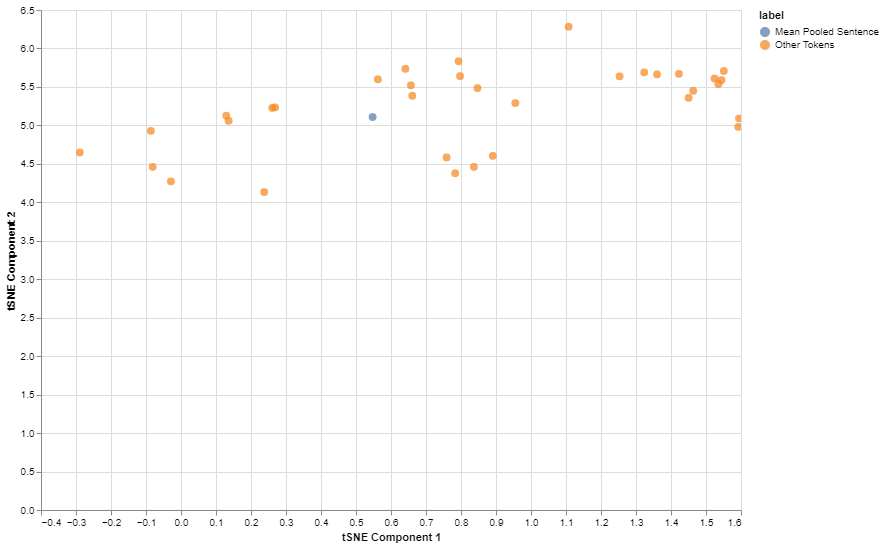
\includegraphics[width=0.9\columnwidth]{oneSentenceLang_lastLayer_tsne.png}
\caption{tSNE visualization of one selected sentence of one selected language on last layer.}
\end{figure}

\subsubsection{Results}

Upon applying tSNE and PCA to token representations and mean-pooled token representations for a sample sentence, several noteworthy observations were made. The mean-pooled representation effectively captured the central tendencies of token representations, residing at the center of the lower-dimensional space. As layers progressed, token representations showed improved separation, forming distinct clusters for semantically different categories. PCA exhibited superior separation, particularly in final layers, producing clearer clusters compared to tSNE.

These observed patterns can be attributed to the hierarchical nature of the language model's feature representations and the characteristics of dimensionality reduction techniques. The mean-pooled representation aggregates semantic information from all tokens, providing a holistic view of the sentence. Improvement in separation across layers suggests hierarchical refinement of features, leading to more distinct representations for tokens with different meanings. PCA's superior performance is due to its linear nature and emphasis on global variance, making it effective in capturing underlying structure, especially in linearly separable final layers. 

Overall, the results highlight the effectiveness of mean-pooled representations in capturing sentence semantics and the importance of considering characteristics of dimensionality reduction techniques when interpreting lower-dimensional representations.

\subsection{Visualizations (all sentences, all languages)}


\begin{figure}[ht]
\centering
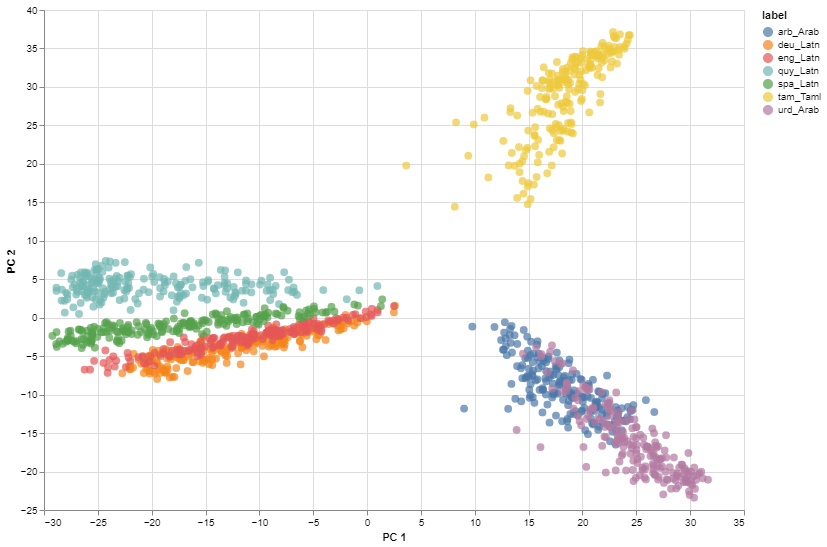
\includegraphics[width=0.9\columnwidth]{allSentenceLang_firstLayer_pca.png}
\caption{PCA visualization of all sentences and all languages on 1st layer.}
\end{figure}


\begin{figure}[ht]
\centering
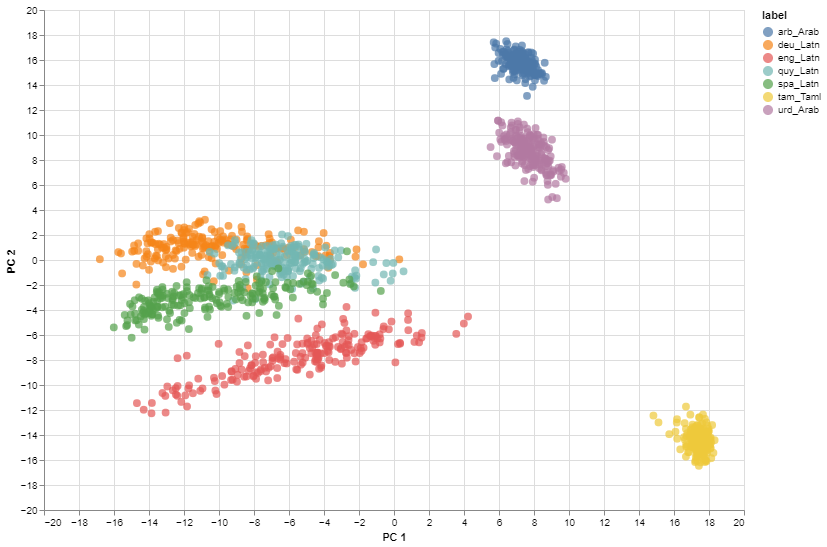
\includegraphics[width=0.9\columnwidth]{allSentenceLang_lastLayer_pca.png}
\caption{PCA visualization of all sentences and all languages on last layer.}
\end{figure}


\begin{figure}[ht]
\centering
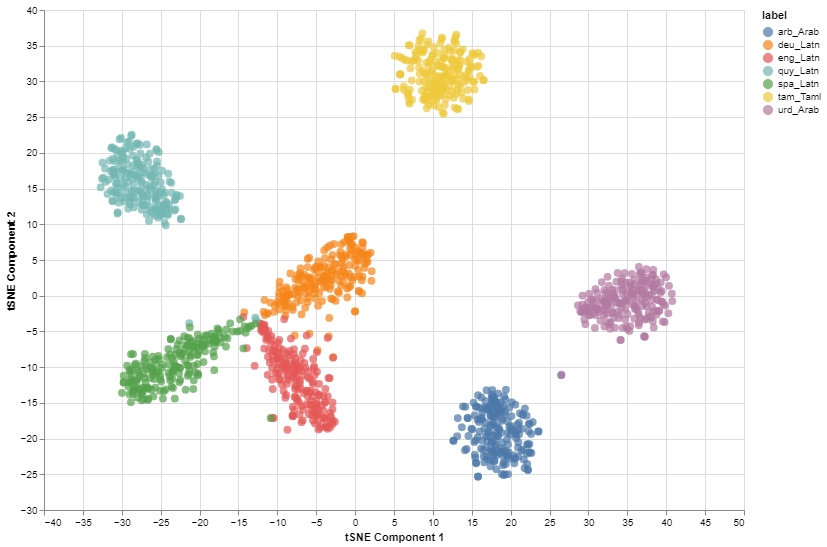
\includegraphics[width=0.9\columnwidth]{allSentenceLang_firstLayer_tsne.png}
\caption{tSNE visualization of all sentences and all languages on 1st layer.}
\end{figure}


\begin{figure}[ht]
\centering
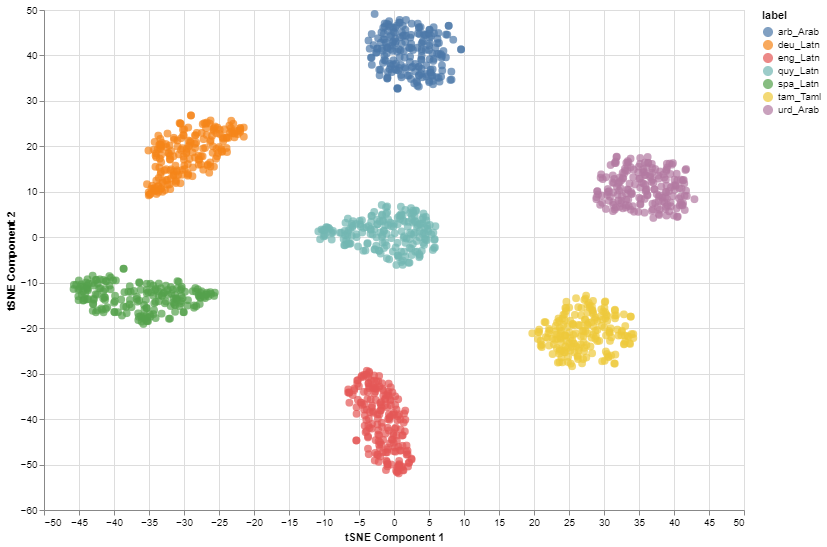
\includegraphics[width=0.9\columnwidth]{allSentenceLang_lastLayer_tsne.png}
\caption{tSNE visualization of all sentences and all languages on last layer.}
\end{figure}

\subsubsection{Results}

Upon applying tSNE and PCA to all mean-pooled token representations for all sentence examples across multiple languages, several significant observations emerged. The resulting lower-dimensional representations exhibited distinct clusters corresponding to the languages to which the sentences belonged, effectively capturing language-specific semantic characteristics. As layers progressed, separation between language clusters improved, with tighter grouping of points from the same language.

These observed patterns can be attributed to the hierarchical nature of the language model's feature representations and the characteristics of dimensionality reduction techniques. Mean-pooled token representations provide a comprehensive view of language-specific characteristics encoded within the tokens. Improvement in separation across layers suggests hierarchical refinement of features, leading to more discriminative representations for sentences in different languages.

tSNE demonstrated better separation of language clusters, especially in the final layers, due to its non-linear nature and emphasis on preserving local relationships. In contrast, PCA's performance was less defined in the final layers, potentially struggling with non-linear relationships and local similarities.

Overall, the results highlight the effectiveness of mean-pooled token representations in capturing language-specific semantic characteristics and the importance of considering characteristics of dimensionality reduction techniques when interpreting lower-dimensional representations.

\section{Task 3: Language model adaptation and Fine tuning}

\subsection{Methodology}

\subsubsection{Dataset Selection}

For the fine-tuning task, the Wikipedia Quechua dataset was chosen as the primary source of training data. This dataset was selected due to its widespread usage and credibility within the community, as evidenced by its large number of downloads. Furthermore, the diversity of content within the dataset, stemming from various sections of Wikipedia pages, presents a challenge for the model to generalize effectively across different domains of Quechua language.

\subsubsection{Fine-tuning Procedure}

The fine-tuning process involves adapting the pre-trained XGLM model on the selected Quechua dataset to improve its performance specifically on Flores Quechua sentences. 

Initially, a full parameter fine-tuning approach was employed, wherein all parameters of the pre-trained model are updated during training. Throughout this process, careful monitoring of the model's performance on a separate test dataset, namely Flores Quechua, is conducted to assess improvements in inference accuracy and language modeling capabilities. 

One noteworthy observation is the negative change in language clustering for the fine-tuned model shown in Figures \ref{vis_ft_pca} and \ref{vis_ft_tSNE}. This is expected as the model gets over-specialized on Quechua at the expense of the model's distinguishing ability across unseen data for other languages .


\begin{figure}[ht]
\centering
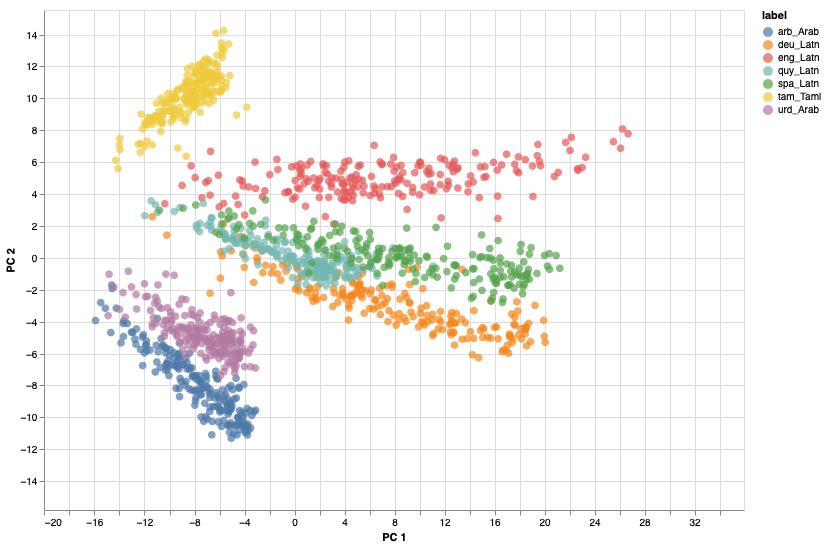
\includegraphics[width=0.9\columnwidth]{visualization_ft_pca.png}
\caption{PCA visualization of all sentences and all
languages on last layer of fine-tuned model.}
\label{vis_ft_pca}
\end{figure}


\begin{figure}[ht]
\centering
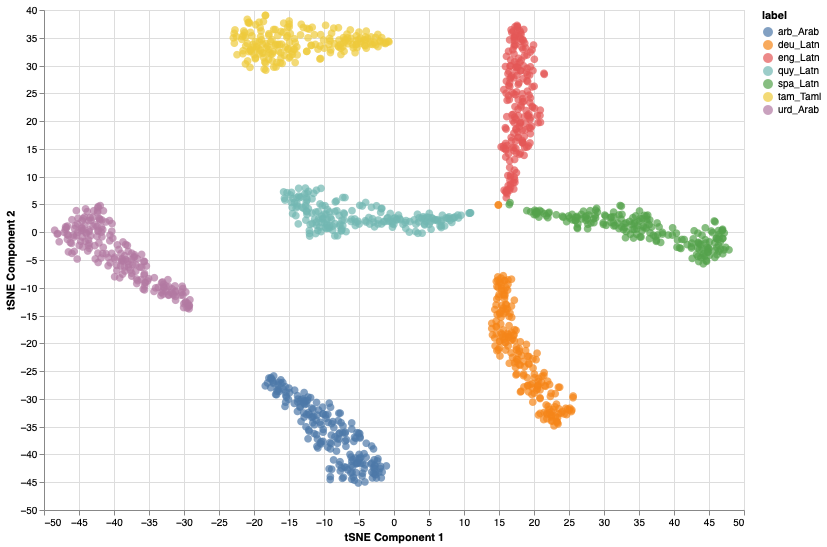
\includegraphics[width=0.9\columnwidth]{visualization_ft_tsne.png}
\caption{tSNE visualization of all sentences and all
languages on last layer of fine-tuned model.}
\label{vis_ft_tSNE}
\end{figure}






\subsubsection{Parameter-Efficient Fine-tuning (PEFT)}

Recognizing the inefficiency associated with fine-tuning all parameters of a large language model, parameter-efficient fine-tuning (PEFT) strategies were explored.

\textbf{BitFit}\cite{zaken2022bitfit}: This approach involves freezing all weights of the transformer model while learning only biases, except for the final fully connected head, where both weights and biases remain unfrozen. By selectively updating parameters, BitFit aims to achieve efficient adaptation while minimizing computational overhead.

\textbf{LoRA}\cite{hu2021lora}: Low-Rank Adaptation (LoRA) maintains the original parameters of the model frozen while introducing an additional low-rank weight matrix to the Query and Value linear layers of the attention modules. This supplementary matrix, being low-rank, effectively reduces the number of trainable parameters, facilitating faster adaptation without compromising model performance significantly.

\textbf{iA3}\cite{liu2022fewshot}: In the iA3 approach, modifications are made to the decoder layers of the XGLM model to scale the keys and values of attention layers by additional learnable parameters. Additionally, the activation of the first fully-connected head in each encoder/decoder block is adjusted. By selectively scaling attention mechanisms, iA3 aims to enhance the model's adaptability to language-specific nuances without overfitting to the training data.

These parameter-efficient fine-tuning strategies offer alternative avenues for adapting the XGLM model to Quechua language data while mitigating computational and memory constraints associated with full parameter fine-tuning.

\subsection{Results}
The results from full-parameter fine-tuning indicate that the mean loss per language(on the Flores devtest split) including Quechua, is generally significantly lower compared to the losses from pretrained XGLM model as shown in Figure \ref{loss_ft}.

BitFit also performs comparably well to full-parameter fine-tuning, giving us an advantage in terms of lower training time.   

Full-parameter fine-tuning, despite its extensive adaptation of parameters, is generally not the best approach for LM adaptations as comparable, task-specific results can be obtained by other parameter-efficient approaches discussed above. LoRA with a rank of 8, also seems to improve the loss on Quechua language significantly, making it the most efficient on the specific task (Causal inference on Quechua). iA3 fine-tuning achieves similar task-specific improvements as well. Table \ref{runtimes} summarises the training times for the above fine-tuning approaches. 


% Please add the following required packages to your document preamble:
% \usepackage{booktabs}
% \usepackage[normalem]{ulem}
% \useunder{\uline}{\ul}{}
\begin{table}[]
\begin{tabular}{@{}ccl@{}}
\toprule
{\ul \textbf{Approach}} & {\ul \textbf{Training time (s)}} & {\ul \textbf{Mean Test loss}} \\ \midrule
Full-parameter          & 3878                             & \textbf{3.502}                          \\
BitFit                  & 3124                             & 3.591                                   \\
LoRA                    & 2322                             & 6.941                                   \\
iA3                     & \textbf{2289}                    & 7.493                                   \\ \bottomrule
\end{tabular}
\caption{Training times and mean test losses on Flores DevTest split.}
\end{table}


\begin{figure}[ht]
\centering
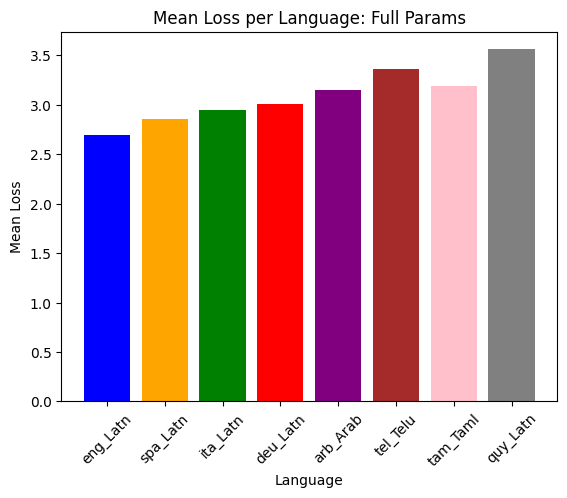
\includegraphics[width=0.9\columnwidth]{loss_ft.png}
\caption{Flores losses on fully fine-tuned model.}
\label{loss_ft}
\end{figure}

\begin{figure}[ht]
\centering
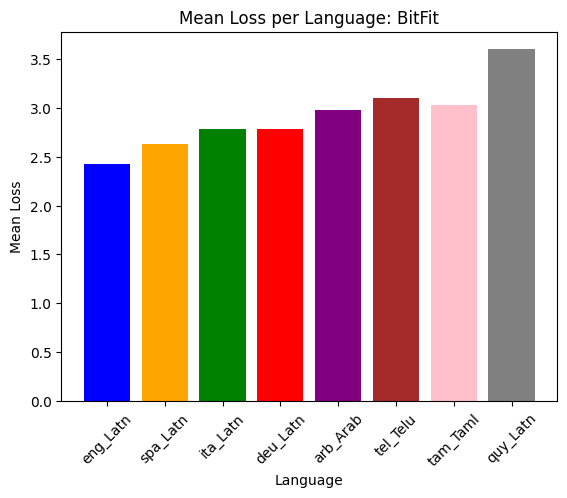
\includegraphics[width=0.9\columnwidth]{loss_bitfit.png}
\caption{XGLM losses after BitFit fine-tuning.}
\label{loss_bitfit}
\end{figure}

\begin{figure}[ht]
\centering
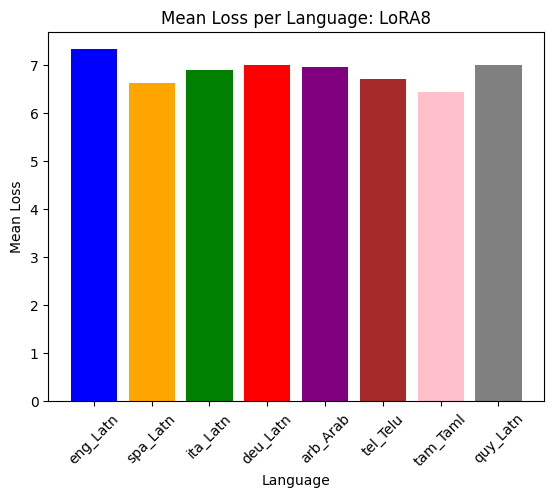
\includegraphics[width=0.9\columnwidth]{loss_lora8.png}
\caption{XGLM losses after LoRA fine-tuning.}
\label{loss_lora}
\end{figure}

\begin{figure}[ht]
\centering
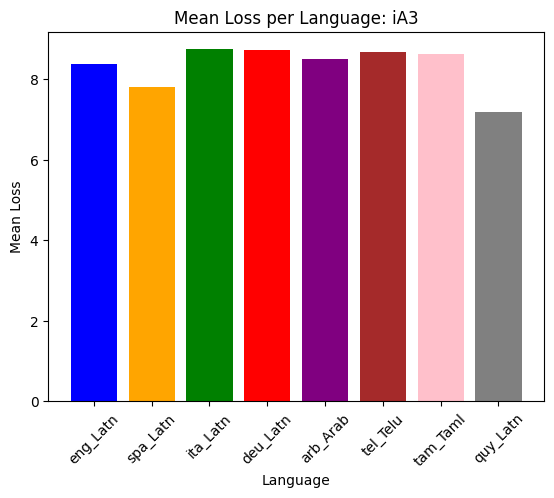
\includegraphics[width=0.9\columnwidth]{loss_iA3.png}
\caption{XGLM losses after iA3 fine-tuning.}
\label{loss_iA3}
\end{figure}


\newpage
\bibliographystyle{plainnat} % Specify bibliography style
\bibliography{references} % Specify path to your .bib file without the extension




\end{document}
